%
% Niniejszy plik stanowi przykład formatowania pracy magisterskiej na
% Wydziale MIM UW.  Szkielet użytych poleceń można wykorzystywać do
% woli, np. formatujac wlasna prace.
%
% Zawartosc merytoryczna stanowi oryginalnosiagniecie
% naukowosciowe Marcina Wolinskiego.  Wszelkie prawa zastrzeżone.
%
% Copyright (c) 2001 by Marcin Woliński <M.Wolinski@gust.org.pl>
% Poprawki spowodowane zmianami przepisów - Marcin Szczuka, 1.10.2004
% Poprawki spowodowane zmianami przepisow i ujednolicenie 
% - Seweryn Karłowicz, 05.05.2006
% Dodanie wielu autorów i tłumaczenia na angielski - Kuba Pochrybniak, 29.11.2016

% dodaj opcję [licencjacka] dla pracy licencjackiej
% dodaj opcję [en] dla wersji angielskiej (mogą być obie: [licencjacka,en])
\documentclass[en]{pracamgr}

% Dane magistranta:
\autor{Katarzyna Kowalska}{371053}

% Dane magistrantów:
%\autor{Autor Zerowy}{342007}
%\autori{Autor Pierwszy}{342013}
%\autorii{Drugi Autor-Z-Rzędu}{231023}
%\autoriii{Trzeci z Autorów}{777321}
%\autoriv{Autor nr Cztery}{432145}
%\autorv{Autor nr Pięć}{342011}

\title{Approximation and Parametrized Algorithms for Segment Set Cover}
\titlepl{Algorytmy parametryzowania i
trudność aproksymacji problemu pokrywania zbiorów
odcinkami na płaszczyźnie}

%\tytulang{An implementation of a difference blabalizer based on the theory of $\sigma$ -- $\rho$ phetors}

%kierunek: 
% - matematyka, informacyka, ...
% - Mathematics, Computer Science, ...
\kierunek{Computer Science}

% informatyka - nie okreslamy zakresu (opcja zakomentowana)
% matematyka - zakres moze pozostac nieokreslony,
% a jesli ma byc okreslony dla pracy mgr,
% to przyjmuje jedna z wartosci:
% {metod matematycznych w finansach}
% {metod matematycznych w ubezpieczeniach}
% {matematyki stosowanej}
% {nauczania matematyki}
% Dla pracy licencjackiej mamy natomiast
% mozliwosc wpisania takiej wartosci zakresu:
% {Jednoczesnych Studiow Ekonomiczno--Matematycznych}

% \zakres{Tu wpisac, jesli trzeba, jedna z opcji podanych wyzej}

% Praca wykonana pod kierunkiem:
% (podać tytuł/stopień imię i nazwisko opiekuna
% Instytut
% ew. Wydział ew. Uczelnia (jeżeli nie MIM UW))
\opiekun{dr Michał Pilipczuk\\
  Instytut Informatyki\\
  }

% miesiąc i~rok:
\date{June 2020}

%Podać dziedzinę wg klasyfikacji Socrates-Erasmus:
\dziedzina{ 
%11.0 Matematyka, Informatyka:\\ 
%11.1 Matematyka\\ 
%11.2 Statystyka\\ 
11.3 Informatyka\\ 
%11.4 Sztuczna inteligencja\\ 
%11.5 Nauki aktuarialne\\
%11.9 Inne nauki matematyczne i informatyczne
}

%Klasyfikacja tematyczna wedlug AMS (matematyka) lub ACM (informatyka)
\klasyfikacja{D. Software\\
  D.127. Blabalgorithms\\
  D.127.6. Numerical blabalysis}

% Słowa kluczowe:
\keywords{set cover, geometric set cover, FPT, W[1]-completeness,
APX-completeness, PCP theorem, NP-completeness}

% Tu jest dobre miejsce na Twoje własne makra i~środowiska:

\newcommand{\points}{\mathcal{C}}
\newcommand{\sets}{\mathcal{P}}
\newcommand{\sol}{\mathcal{R}}
\newcommand{\then}{\Rightarrow}

\newcommand{\xTrueSegment}{(c_i, g_i)}
\newcommand{\xFalseSegment}{(f_i, h_i)}

\usepackage{amsfonts}
\usepackage{amsmath}
\usepackage{graphicx}
\usepackage{xcolor}
\usepackage[nospace, noadjust]{cite}
\usepackage{lineno}
\linenumbers

\newtheorem{claim}{Claim}[section]
\newtheorem{defi}{Definition}[section]
\newtheorem{tw}{Theorem}[section]
\newtheorem{lemma}{Lemma}[section]

\setcounter{secnumdepth}{3}
\setcounter{tocdepth}{3}


% koniec definicji

\begin{document}
\maketitle

%tu idzie streszczenie na strone poczatkowa
\begin{abstract}
  The work presents a study
  of different geometric set cover problems.
  It mostly focuses on segment set cover
  and its connection to the polygon set cover.
\end{abstract}

\tableofcontents
%\listoffigures
%\listoftables

\chapter{Introduction}

The Set Cover problem is one of the most common NP-complete problems.
[tutaj referencja]
We are given a family of sets and have to choose the smallest
subfamily of these sets that cover all their elements.
This problem naturally extends to settings
were we put different weights on the sets
and look for the subfamily of the minimal weight.
This problem is NP-complete even 
without weights and if we put
restrictions on what the sets can be.
One of such variants is Vertex Cover problem,
where sets have size 2 (they are edges in a graph).

In this work we focus on another such variant where the sets correspond
to some geometric shapes and
only some points of the plane have to be covered.
When these shapes are rectangles with edges parallel
to the axis, the problem can be proven to
be W[1]-complete (solution of size $k$ cannot be found
in $n^o(k)$ time),
APX-complete (for suffciently small $\epsilon > 0$, the problem
does not admit $1+\epsilon$-approximation scheme)
[refrencje].

Some of these settings are very easy.
Set cover with lines parallel to one of the axis
can be solved in polynomial time.

There is a notion of $\delta$-expansions,
which loosen the restrictions on geometric set cover.
We allow the objects to cover the points
after $\delta$-expansion and compare
the result to the original setting.
This way we can produce both FPT and EPTAS
for the rectangle set cover with $\delta$-extensions
[referencje].



\paragraph{Our contribution.}
In this work, we prove that unweighted geometric set cover
with segments is fixed parameter tractable (FPT).

Moreover, we show that geometric set cover with segments
is APX-complete for unweighted axis-parallel segments,
even with 1/2-extensions.
So the problem for very thin rectangles
also can't admit PTAS.
Therefore, in the efficient polynomial-time approximation scheme (EPTAS)
for \textit{fat polygons} by \cite{harpeled12},
the assumption about polygons being fat is necessary. 

Finally, we show that geometric set cover with weighted segments in
3 directions is W[1]-complete.
However, geometric set cover with weighted segments is FPT if we allow
$\delta$-extension.

This result is especially interesting,
since it's counter-intuitive that
the unweighed setting is FPT and the weighted
setting is W[1]-complete.
Most of such problems (like vertex cover or [wiecej przykladow])
are equally hard in both weighted and unweighted settings.

\chapter{Definitions}
Some definitions what geometric set cover is.
$\sets$ -- set of objects, $\points$ -- set of points.
Choose $\sol \subset \sets$ such that
every point in $\points$ is inside some element from $\sol$
and $|\sol|$ is minimal.

In parametrized setting we only look among $|\sol| \le k$.
In weighted settings there is some $f : \sets -> \mathbb{R}$
and we minimize $\sum_{R \in \sol} f(R)$.

\chapter{Geometric Set Cover with segments}

\section{FPT for segments}
\subsection{Segments parallel to one of the axis}
You can find this in Platypus book.

We'll show $\mathcal{O}(2^k)$ branching algorithm.
Let's take point $K$ that hasn't been covered yet with
the smallest coordinate in lexicograpical order.
We need to cover $K$ with some of the remaining segments.

We choose one of the 2 directions on which we cover this point.
In this direction we take greedly the segment that will cover
the most points (there are points in $\points$ only on
one side of $K$ in this direction, so all
segments covering $K$ in this direction create monotone sequence
of sets -- zbiory zstępujące).

\subsection{Segments in $d$ directions}
The same algorithm as before but in complexity $\mathcal{O}(d^k)$.

\subsection{Segments in arbitrary direction}
\begin{tw}{
	\label{segment_cover_fpt}
	\textbf{(FPT for segment cover)}.
	There exists an algorithm that given a family $\sets$ of
	$n$ segments (in any direction),
	a set of $m$ points $\points$
	and a parameter $k$,
	runs in time $f(k) \cdot (nm)^c$ for some computable function f and constant c,
	and outputs a subfamily $\sol \subseteq \sets$
	such that $|\sol| \le k$ and $\sol$ covers all points in $\points$
	or determins that the solution of size at most $k$ doesn't exist.
}\end{tw}

This theorem is proved by following lemmas.

\begin{lemma}
   \label{fpt_reduction}
   \textbf{(Reduction)}.
   Given a family $\sets$ of
	$n$ segments (in any direction),
	a set of $m$ points $\points$
	for segment cover problem,
   without a loss of generality we can assume that
   no two segments cover the same set of points.
\end{lemma}   
   
\paragraph{Proof.} Trivial.

\begin{lemma}
	\label{kernel_definition}
	\textbf{(Kernel for segment cover)}.
	For a problem of segment cover that given a family $\sets$ of
	$n$ segments (in any direction),
	a set of $m$ points $\points$
	and a parameter $k$, there exists a family of
	kernels $K \subset \sets$,
	where \textit{any line} contains no more than $k$ points
	and there exists optimal solution, that is subset of $K$.
	We can find all such kernels in complexity $O(k^k)$ using branching technique
	and there are $O(k^k)$ of them.
\end{lemma}

\paragraph{Proof.}

%As long as there is a line with more than $k$ points, do branching.
%Let's name points on this line $x_1, x_2, \ldots x_t$
%in order they appear on the line.

%So we choose on which point the chosen segment on this line
%will start. Of course we have to take at least one segment
%covering at least one point among first $k+1$ points,
%because covering all of them with only segments
%on different lines we would use
%exactly $k+1$ segments (any of them can't contain more than
%one point from this line).

First we use Lemma \ref{fpt_reduction}.

Assume there exists a line $l$ containing points $x_1$, \ldots $x_t$,
where $t \geq k + 1$.
Note that a segment that does not lie on $l$ can cover only at most one
of the points $x_i$.
Therefore, out of points $x_1$, ..., $x_{k+1}$,
at least one has to be covered by a segment that lies on $l$,
let us fix $x_i$ to be the first such point (We branch over $i \in \{1 \dots k+1\}$.
Then, we can greedily choose a segment that lies on $l$,
covers $x_i$,
and also covers the largest number of points $x_j$ for $j > i$.

Since we have at most $k + 1$ choices to branch over
and each choice adds a segment to the constructed solution,
we obtain an algorithm with complexity $O(k^k)$.

\paragraph{Proof of theorem \ref{segment_cover_fpt}.} Assuming Lemma \ref{kernel_definition}.

First we use Lemma \ref{fpt_reduction}.

Since any segment covers a set of colinear points,
for such a kernel $k$ segments can cover only at most $k^2$ points.
Therefore, for the answer to be positive,
the number of points has to be at most $k^2$.
The number of segments is now bounded by $k^4$,
since if we consider two \textit{extreme} points
covered by a given segment,
then these pairs must be distinct,
otherwise two segments would contain the same set of points.
Since both the number of points and the number of segments
is bounded by a function of $k$,
this instance can be easily solved in time $O(f(k))$.
Since there are $O(k^k)$ possible kernels, the final algotihm
work in $f(k) \cdot (nm)$.

\section{APX-completeness for segments parallel to axes}
\label{section:segment_apx}

In this section we analyze whether there exists 
PTAS for geometric set cover for rectangles.
We show that we can restrict this problem
to a very simple setting:
segments parallel to axes and allow (1/2)-extension,
and the problem is still APX-hard.
Note that segments are just degenerated rectangles
with one side being very narrow.


Our results can be summarized in the following
theorem and this section aims to prove it.

\begin{tw}{
\label{segment_cover_apx_hard}
	\textbf{(axis-parallel segment set cover with 1/2-extension is APX-hard)}.	
	Unweighted geometric set cover
	with axis-parallel segments in 2D (even with 1/2-extension)
	is APX-hard.
	That is, assuming $P\neq NP$, there does not exist a PTAS
	for this problem.
}\end{tw}
 
Theorem \ref{segment_cover_apx_hard} implies the following.

\begin{corollary}{
\label{rectangle_cover_apx_hard}
	\textbf{(rectangle set cover is APX-hard)}.	
	Unweighted geometric set cover
	with rectangles (even with 1/2-extension) is APX-hard.
}\end{corollary}


We prove Theorem \ref{segment_cover_apx_hard}
by taking a problem that is APX-hard
and showing a reduction.
For this problem we choose
MAX-(3,3)-SAT which we define below.


\subsection{MAX-(3,3)-SAT and statement of reduction}
\begin{defi}
\textbf{MAX-3SAT} is the following maximization problem. We are given a 3-CNF
formula, and need to find an assignment of variables
that satisfies the most clauses.
\end{defi}

\begin{defi}
\textbf{MAX-(3,3)-SAT} is a variant of MAX-3SAT with an additional
restriction that every variable appears in exactly 3 clauses.
Note that thus, the number of clauses is equal to the number of variables.
\end{defi}

In our proof of Theorem \ref{segment_cover_apx_hard} we use
hardness of approximation of MAX-(3,3)-SAT proved
in \cite{hastad} and described in
Theorem \ref{hastadtheorem} below.

\begin{defi}[$\alpha$-satisfiable MAX-3SAT formula]
MAX-3SAT formula of size $n$ is at most $\alpha$-satisfiable, if
every assignment of variables satisfies no more than $\alpha n$
clauses. 
\end{defi}

\begin{tw}{
	\label{hastadtheorem}
	\textbf{\cite{hastad}}
	
	For any $\epsilon > 0$, it is NP-hard to distinguish satisfiable
	(3,3)-SAT formulas from
	%This broke x-satisfiable to next line
	at most
	\linebreak\mbox{$(7/8 + \epsilon)$-satisfiable}
	(3,3)-SAT formulas.
}\end{tw}


Given an instance $I$ of MAX-(3,3)-SAT,
we construct an instance $J$ of 
axis-parallel segment set cover problem,
such that for a sufficiently small $\epsilon > 0$,
a polynomial time $(1+\epsilon)$-approximation algorithm for $J$
would be able to distinguish  whether an instance $I$ of MAX-(3,3)-SAT
is fully satisfiable
or is at most $(7/8 + \epsilon)$-satisfiable.
However, according to (Theorem \ref{hastadtheorem}) the latter problem
is NP-hard.
This would imply P = NP, contradicting the assumption.

The following lemma encapsulates the properties
of the reduction described in this section,
and it allows us to prove Theorem \ref{segment_cover_apx_hard}.

\begin{lemma}{
	\label{apxconstruction}
	Given an instance $S$ of  MAX-(3,3)-SAT 
	with $n$ variables and optimum value $opt(S)$,
	we can construct an instance $I$ of geometric set cover with
	axis-parallel segments in 2D, such that:
	\begin{enumerate}[label={(\arabic*)}]
	\item For every solution $X$ of instance $I$,
	there exists a solution of $S$ that satisfies at least  $15n - |X|$
	clauses.
	
	\item For every solution of instance $S$ that satisfies $w$ clauses,
	there exists a solution of $I$ of size $15n - w$.
	
	\item Every solution with $1/2$-extensions of $I$
	is also a solution to the original instance $I$.
		
	Therefore, the optimum size of a solution of $I$
	is $opt(I) = 15n - opt(S)$. 
	\end{enumerate}
	
}\end{lemma}

We prove Lemma \ref{apxconstruction} in
subsequent sections, but meanwhile let us prove
Theorem \ref{segment_cover_apx_hard} using Lemma \ref{apxconstruction}
and Theorem \ref{hastadtheorem}.

TODO: This below can't use current template

\begin{proof}[Proof of Theorem \ref{segment_cover_apx_hard}].
Consider any $0 < \epsilon < 1/(15 \cdot 8)$.

Let us assume that there exists a polynomial-time
$(1+\epsilon)$-approximation algorithm
for unweighted geometric set cover with axis-parallel segments in 2D
with (1/2)-extensions.
We construct an algorithm that solves the problem stated in 
Theorem \ref{hastadtheorem}, thereby proving that P = NP.

Take an instance~$S$ of MAX-(3,3)-SAT to be distinguished
and construct an instance of geometric set cover $I$
using Lemma \ref{apxconstruction}.
We now use the $(1+\epsilon)$-approximation algorithm
for geometric set cover on $I$.
Denote the size of the solution returned by this algorithm as $approx(I)$.
We prove that 
if in $S$
one can satisfy at most $(\frac{7}{8}+\epsilon)n$ clauses,
then $approx(I) \ge 15n - (\frac{7}{8} + \epsilon)n$
and if $S$ is
satisfiable, then $approx(I) < 15n - (\frac{7}{8} + \epsilon)n$.

\subparagraph{Assume $S$ satisfiable.}
From the definition of $S$ being satisfiable, we have:
$$opt(S) = n.$$

From Lemma \ref{apxconstruction} we have:

$$opt(I) = 14n.$$

Therefore,
$$approx(I) \le (1+\epsilon)opt(I) = 14n(1+\epsilon)
	= 14n + 14\epsilon\cdot n =$$ 
	$$= 14n + (15\epsilon - \epsilon)n < 
  14n + \left(\frac{1}{8} - \epsilon\right)n 
= 15n - \left(\frac{7}{8} + \epsilon\right)n$$

\subparagraph{Assume $S$ is at most 
$\left(\frac{7}{8} + \epsilon\right)$ satisfiable.}
From the defintion of $S$ being at most 
$\left(\frac{7}{8} + \epsilon\right)n$ satisfiable, we have:
$$opt(S) \le \left(\frac{7}{8} + \epsilon\right)n$$

From Lemma \ref{apxconstruction} we have:
$$opt(I) \ge 15n - \left(\frac{7}{8} + \epsilon\right)n$$

Since a solution to $I$ with $\frac{1}{2}$-extensions is
also a solution without extentions, by 
Lemma \ref{apxconstruction} (3.), we have:

$$approx(I) \ge opt(I) = 15n - \left(\frac{7}{8} + \epsilon\right)n$$


Therefore, by using the assumed $(1+\epsilon)$-approximation
algorithm,
it is possible to distinguish the case when
$S$ is satisfiable from the case when it is
at most $(\frac{7}{8} + \epsilon)n$ satisfiable,
it suffices to compute $approx(I)$ with $15n - (\frac{7}{8}+\epsilon)n$.
Hence, the assumed approximation algorithm cannot exist, unless P = NP.

\end{proof}

\subsection{Reduction construction}
\label{construction_description}
We show reduction from MAX-(3,3)-SAT problem
to geometric set cover with segments
parallel to axis. Moreover the instance
of geometric set cover will be robust
to 1/2-extensions (have the same optimal solution
after 1/2-extension).

The construction will be composed of 2 types of gadgets:
\textbf{VARIABLE-gadgets} and \textbf{CLAUSE-gadgets}.
CLAUSE-gadgets would be constructed using two \textbf{OR-gadgets}
connected together.


\subsubsection{VARIABLE-gadget}

VARIABLE-gadget is responsible for choosing the value of a variable
in a CNF formula. It allows two minimal solutions
and every minimal solution must use exactly one of the
$\xTrueSegment$ and $\xFalseSegment$
segments. These two choices correspond to the two Boolean values of the variable.

\paragraph{Points.}

Define points:
\begin{figure}[h]
\centering
\def\svgwidth{0.5\columnwidth}
\input{apx_choose_variable.pdf_tex}
\caption{\textbf{VARIABLE-gadget.}
We denote the set of points marked with black circles as $C_{var}^i$,
and they need to be covered (are part of the set $\points$).
Note that some of the points are not marked as black dots
and exists only to name segments for further reference.
We denote the set of red segments as $X_{false}^i$
and the set of green segments as $X_{true}^i$.}
\label{fig:apx_choose_variable}
\end{figure}

With $L = 12n$:

\begin{center}
\begin{tabular}{ l l l l}
	$a = (-L, 0)$ &
	$b = (-\frac{2}{3}L, 0)$ & 
	$c = (-\frac{1}{3}L, 0)$ & 
	$d = (-L, 1)$ \\  
	$e = (-\frac{2}{3}L, 1)$ & 
	$f = (-\frac{2}{3}L, 2)$ &
	$g = (L, 0)$ &
	$h = (L, 2)$
\end{tabular}
\end{center}

Let us define: $$C_{var} =  \{a, b, c, d, e, f\}$$
and $$C_{var}^i = C_{var} + (0, 4i)$$


\paragraph{Segments.}

Let us define:

$$X_{true}^i =\{ (a_i, d_i), (b_i, f_i), (c_i, g_i)\}$$
$$X_{false}^i = \{(a_i, c_i), (d_i, e_i), (f_i, h_i)\}$$

$$P_{var}^i = X_{true}^i \cup X_{false}^i$$


\begin{lemma}
\label{choose_variables_solution}
For any $1 \le i \le n$, points $C_{var}^i$
can be covered using 3 segments from $P_{var}^i$.
\end{lemma}

\begin{proof}
We can use either set $X_{true}^i$ or $X_{false}^i$.
\end{proof}

\begin{lemma}
\label{choose_variables_no_less}
For any $1 \le i \le n$, points $C_{var}^i$
can not be covered with less than 3 segments from $P_{var}^i$.
\end{lemma}

\begin{proof}
No segment of $P_{var}^i$ covers more than one point from
$\{d_i, f_i, c_i\}$, therefore $C_{var}^i$ can
not be covered with less than 3 segments.
\end{proof}

\begin{lemma}
\label{choose_variables_both}
For every set $A \subseteq P_{var}^i$, such that $A$ covers $C_{var}^i$
and $\xTrueSegment \in A, \xFalseSegment \in A$,
it holds that $|A| \ge 4$.
\end{lemma}
\begin{proof}
No segment from $P_{var}^i$ covers more than one point from
$\{a_i, e_i\}$,
therefore 
$C_{var}^i$ - $\{c_i, f_i, g_i, h_i\}$
can not be covered with less than 2 segments.
\end{proof}


\subsubsection{OR-gadget}

OR-gadget has 3 important segments
-- $x, y, result$. $x$ and $y$ don't count to the weight of solution
of OR-gadget (they are part of different gadgets).
It has a minimal solution of weight $w$
and $result$ can be chosen only if $x$ or $y$ are also chosen
for the solution.
If none of them are chosen, then solution
choosing $result$ segment has weight at least $w+1$.
Therefore the following formula holds for a solution $R$
assuming that $R$ uses only $w$ from this OR-gadget:

$$ (x \in R) \lor (y \in R) \iff result \in R  $$

\paragraph{Points.}

\begin{figure}[h]
\centering
\def\svgwidth{0.5\columnwidth}
\input{apx_or_gadget.pdf_tex}
\caption{
\textbf{OR-gadget.} We denote these point as $or\_gadget_{i, j}$. 
We denote set of red segments as $or^{false}_{i, j}$,
set of blue segments as $or^{true}_{i, j}$,
green and yellow segments as $or\_move\_variable_{i, j}$.
}
\label{fig:apx_or_gadget}
\end{figure}

	\begin{center}
\begin{tabular}{ l l l l}

	$l_0 = (0, 0)$ &
	$m_0 = (0, 1)$ &
	$n_0 = (0, 2)$ &
	$o_0 = (0, 3)$ \\
	$p_0 = (0, 4)$ &
	$q_0 = (1, 1)$ &
	$r_0 = (1, 3)$ &
	$s_0 = (2, 1)$ \\
	$t_0 = (2, 2)$ &
	$u_0 = (2, 3)$ &
	$v_0 = (3, 2)$ &
\end{tabular}
\end{center}


	$$vec_{i, j} = (10i + 3 + 3j, 4n + 2j)$$
	
	Define 
	$\{ l_{i, j}, m_{i, j} \ldots v_{i, j} \}$
	as $\{l_0, m_0 \ldots v_0\}$ shifted by $vec_{i, j}$

Note that $v_{i, 0} = l_{i, 1}$ (see Figure~\ref{fig:apx_clause})
 
  $$C\_or\_gadget_{i, j} = 
 \{l_{i, j}, m_{i, j}, n_{i, j}, o_{i, j},
 p_{i, j}, q_{i, j}, r_{i, j}, s_{i, j}, t_{i, j}, u_{i, j} \}
 $$
 
\paragraph{Segments.}

We define names subsets of segments, to refer to them in lemmas.
 
$$or^{false}_{i, j} =
\{ (q_{i, j}, r_{i, j}), (s_{i, j}, u_{i, j})\}$$
$$or^{true}_{i, j} =
\{ (m_{i, j}, s_{i, j}), (o_{i, j}, u_{i, j}),
(t_{i, j}, v_{i, j}) \}$$

$$or\_move\_variable_{i, j} =
\{ (l_{i, j}, n_{i, j}), (n_{i, j}, p_{i, j})\}$$

Segments in OR-gadget:

$$P\_or\_gadget_{i, j} = 
  or^{false}_{i, j} \cup or^{true}_{i, j} \cup or\_move\_variable_{i, j}
  $$


\begin{lemma}
\label{cover_or_true}
For any $1 \le i \le n, j \in \{0, 1\}$ and 
 $x \in \{l_{i, j}, p_{i, j}\}$ we can cover points in
$C\_or\_gadget_{i, j} - \{ x\} \cup \{v_{i, j}\}$
with 4 segments from $P\_or\_gadget_{i,j}$.
\end{lemma}

\begin{proof}
We can do that using one segment from
$or\_move\_variable_{i, j}$
(chosen depending on the value of $x$)
and all segments from $or^{true}_{i, j}$.
\end{proof}

\begin{lemma}
\label{cover_or_false}
For any $1 \le i \le n, j \in \{0, 1\}$, we can cover points in
$C\_or\_gadget_{i, j}$ with 4 segments from $P\_or\_gadget_{i,j}$.
\end{lemma}

\begin{proof}
We can do that using  $or\_move\_variable_{i, j}$
and $or^{false}_{i, j}$.
\end{proof}


\subsubsection{CLAUSE-gadget}


CLAUSE-gadget is responsible for calculating if choice of the
variable values meets the clause in formula.
It has minimal solution of weight $w$ if at least one variable
in the clause has a correct value.
Otherwise it has minimal solution $w+1$.
This way by the minimal solution for the whole problem, we can tell
how many clauses were satisfiable.

The CLAUSE-gadgets consist of two OR-gadgets.
We don't want the CLAUSE-gadgets to be crammed 
somewhere between
the very long variable segments. That's why we have a simple
gadget to \textit{pass} the value of the segment, ie. segments
$(x_{i, 0}, x_{i, 1}), (y_{i, 0}, y_{i, 1}), (z_{i, 0}, z_{i, 1})$.
Two segments and one of them is chosen if $x$ was chosen
in the solution and the other one if $x$ wasn't.

\paragraph{Points.}


\begin{figure}[h]
\centering
\def\svgwidth{0.8\columnwidth}
\input{apx_clause.pdf_tex}
\caption{\textbf{CLAUSE-gadget.}
We denote set of these points as $C\_clause_i$.
Every green rectangle is an OR-gadget.
$y$-coordinates of $x_{i, 0}$, $y_{i, 0}$ and $z_{i,0}$
depend on the values of variables in the $i$-th clause.
}
\label{fig:apx_clause}
\end{figure}

TODO: Rephrase it

Assuming clause $C_i = x_i \lor y_i \lor z_i$,
function $idx(w)$ is returning index of the variable $w$,
function $neg(w)$ is returning whether variable $w$ is negated
in a clause.

\begin{center}
\begin{tabular}{ l l }
	$x_{i, 0} = (10i+1, 4\cdot idx(x_i) + 2\cdot neg(x_i))$ &
	$x_{i, 1} = (10i+1, 4n)$ \\
	$y_{i, 0} = (10i+2, 4\cdot idx(y_i) + 2\cdot neg(y_i))$ &
	$y_{i, 1} = (10i+2, 4n + 4)$ \\
	$z_{i, 0} = (10i+3, 4\cdot idx(z_i) + 2\cdot neg(z_i))$ &
	$z_{i, 1} = (10i+3, 4n + 6)$
\end{tabular}
\end{center}
	
 
 $$move\_variable_i = 
 \{x_{i, j} : j \in \{0, 1\}\} \cup
 \{y_{i, j} : j \in \{0, 1\}\} \cup
 \{z_{i, j} : j \in \{0, 1\}\} 
 $$
 
 $$C\_clause_i = 
 move\_variable_i \cup C\_or\_gadget_{i, 0}
 \cup C\_or\_gadget_{i, 1} \cup \{v_{i, 1} \} 
 $$

\paragraph{Segments.}

\begin{eqnarray*}
P\_clause_i & = & \{ (x_{i, 0}, x_{i, 1}),
(y_{i, 0}, y_{i, 1}),
(z_{i, 0}, z_{i, 1}),
(x_{i, 1}, l_{i, 0}),
(y_{i, 1}, p_{i, 0}),
(z_{i, 1}, p_{i, 1}),
\} \cup \\
& & \cup \ P\_or\_gadget_{i, 0} \cup P\_or\_gadget_{i, 1}
\end{eqnarray*}

\begin{lemma}
\label{cover_clauses_solution_true}
For any $1 \le i \le n$ and $a \in \{ x_{i, 0}, y_{i, 0}, z_{i, 0}\}$,
points $C\_clause_i - \{a\}$ can be covered with $P\_true^a_i \subset P\_clause_i$,
such that $|P\_true^a_i| = 11$.
\end{lemma}

\begin{proof}
For $a = x_{i, 0}$ (analogous proof for $y_{i, 0}$):
First we use Lemma~\ref{cover_or_true} twice with excluded $x = l_{i, 0}$ and
$x = l_{i, 1} = v_{i, 0}$,
resulting with 8 segments $or^{true}_{i, 0} \cup or^{true}_{i, 1}$
which cover all required points apart from
$x_{i, 1}, y_{i, 0}, y_{i, 1}, z_{i, 0}, z_{i, 1}, l_{i, 0}$.
We cover those using additional 3 segments:
$\{ (x_{i, 1}, l_{i, 0}), (y_{i, 0}, y_{i, 1}),
(z_{i, 0}, z_{i, 1}) \}$

For $a = z_{0, i}$:
Using Lemma~\ref{cover_or_false} and Lemma~\ref{cover_or_true} with
$x = p_{i, 1}$,
resulting with 8 segments $or^{false}_{i, 0} \cup or^{true}_{i, 1}$
which cover all required points apart from
$x_{i, 0}, x_{i, 1}, y_{i, 0}, y_{i, 1}, z_{i, 1}, p_{i, 1}$.
We cover those using additional 3 segments:
$\{ (x_{i, 0}, x_{i, 1}), (y_{i, 0}, y_{i, 1}),
(z_{i, 1}, p_{i, 1}) \}$.
\end{proof}

\begin{lemma}
\label{cover_clauses_solution_false}
For any $1 \le i \le n$,
points $C\_clause_i$ can be covered with $P\_false_i \subset P\_clause_i$,
such that $|P\_false_i| = 12$.
\end{lemma}

\begin{proof}
Using Lemma \ref{cover_or_false} twice we can
cover $or\_gadget_{i,0}$ and  $or\_gadget_{i,1}$
with 8 segments.

To cover the remaining points we additionally use:
$\{ (x_{i, 0}, x_{i, 1}), (y_{i, 0}, y_{i, 1}),
(z_{i, 0}, z_{i, 1}), (t_{i, 1}, v_{i, 1}) \}$

\end{proof}

\begin{lemma}
\label{cover_clauses_segments_no_less}
For any $1 \le i \le n$:
\begin{enumerate}[label={(\arabic*)}]
	\item points $C\_clause_i - \{ x_{i, 0}, y_{i, 0}, z_{i, 0}\}$
	can not be covered using less than 11 segments from $P\_clause_i$;
	\item points $C\_clause_i$ can not be covered with less than
	12 segments from $P\_clause_i$.
\end{enumerate}
\end{lemma}


\begin{proof}[Proof of no cover with less than 12 segments.]
There is independent set of 12 points in $C\_clause_i \supseteq
\{ x_{i, 0}, y_{i, 0}, z_{i, 0}, l_{i, 0}, p_{i, 0}, q_{i, 0},
u_{i, 0}, v_{i, 0} = l_{i, 1}, p_{i, 1}, q_{i, 1}, u_{i, 1}, v_{i, 1} \}$.
\end{proof}

\begin{proof}[Proof of no cover with less than 11 segments.]

We can choose disjoint sets $X, Y, Z$ such that
$X \cup Y \cup Z \subseteq C\_clause_i - \{x_{i, 0}, y_{i, 0}, z_{i, 0}\}$
and there are no segments covering points from different sets.
And we prove lower bounds for each of these sets.

$$X = \{x_{i, 1}, y_{i, 1}, z_{i, 1}\}$$

Set $X$ is an indendent set, so it must be covered with 3 segments.

$$Y = or\_gadget_{i, 0} - \{l_{i, 0}, p_{i, 0}\}$$
$$Z = or\_gadget_{i, 1} - \{l_{i, 1}, p_{i, 1}\}$$


For both $Y$ and $Z$ we can check all of the subsets of 3 segments
with brutforce that none of them cover, so they have to be covered with
4 segments.

TODO: Funny fact, neither Y nor Z doesn't have independent set of size 4.

Therefore $C\_clause_i$ must be covered with at least 3 + 4 + 4 = 11 segments.
\end{proof}

\subsubsection{Summary}

Add some smart lemmas that sets will be exclusive to each other.

\begin{lemma}
\textbf{Robustness to 1/2-extensions}. For every segment $s \in \sets$,
$s$ and $s^{+1/2}$ cover the same points from $\points$.
\end{lemma}

\begin{proof}
We can just check every segment. Most of the segments $s$
are colinear only with points that lay on $s$,
so trivially $s^{+1/2}$ cannot cover more points than $s$ does.

TODO: list problematic segments here
\end{proof}


\subsubsection{Summary of construction}

\begin{figure}
\centering
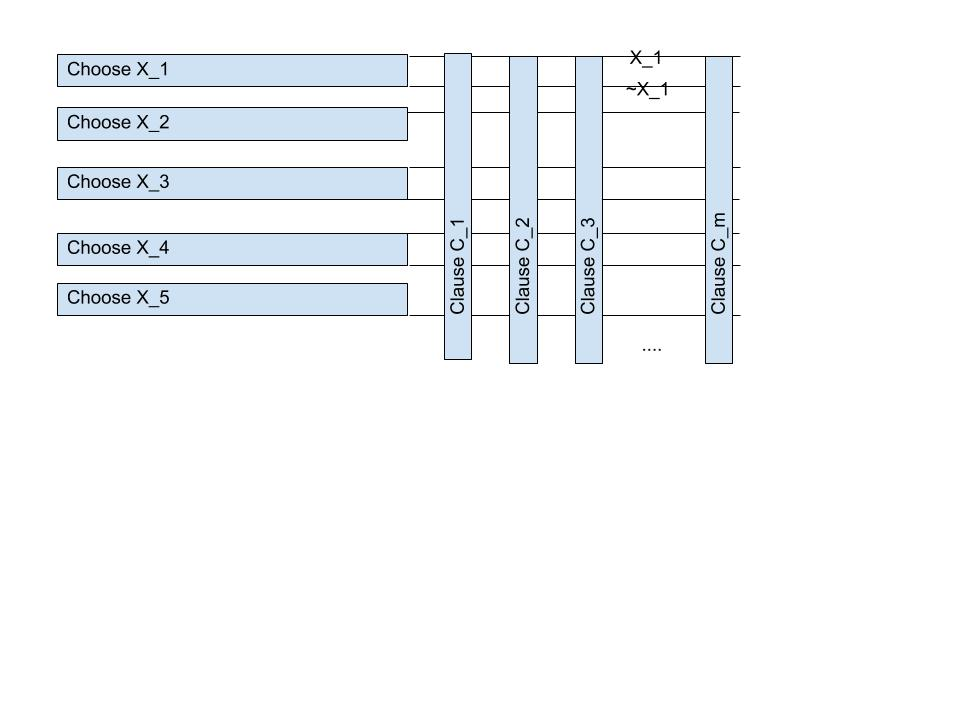
\includegraphics[width=\linewidth]{segment_apx_sketch.jpg}
\caption{\textbf{General schema.}}
General layout of VARIABLE-gadget and CLAUSE-gadget and how they
interact with each other.

TODO: Rename Choose X to VARIABLE-gadget and Clause C to CLAUSE-gadget.
\label{fig:segment_apx_sketch}
\end{figure}

We define:
$$\points := \bigcup_{1 \le i \le n} C\_variable_i \cup C\_clause_i $$
$$\sets := \bigcup_{1 \le i \le n} P\_variable_i \cup P\_clause_i $$

The subsequent sections define these sets.

We prove some properties of different gadgets.
Every segment for a gadget will only cover points 
in this gadget (won't interact with any diferent gadget),
so we can prove lemmas \textit{locally}.


TODO: $y$ axis is increasing values downward on figures
(not upwards like in normal).



\subsection{Construction lemmas and proof of Lemma \ref{apxconstruction}}
\begin{lemma}
	\label{construction_correctness}
	Given an instance $S$ of MAX-(3,3)-SAT of size $n$
	with optimum solution satisfying $k$ clauses $opt(S) = k$.
	Instance of geometric cover, constructed for $S$
	as described in Section~\ref{construction_description}, 
	can be solved with a solution of size $15n - k$.
\end{lemma}

\begin{proof}
Let us name the assignments of the variables in
the optimum solution of an instance $S$ as
$y_1$,~$y_2$~$\ldots$~$y_n$ and clauses as
$c_1$,~$c_2$~$\ldots$~$c_n$.


We cover every VARIABLE-gadget with solution described in
Lemma~\ref{choose_variables_solution},
in the $i$-th gadget choosing the set of segments corresponding to the
value of $y_i$. 
CLAUSE-gadgets that are satisfied,
let us name the variable that is true in them $a$,
are covered with set $P\_true_i^a$ described in
Lemma~\ref{cover_clauses_solution_true}
and unsatisfied with set $P\_false_i$ described in
Lemma~\ref{cover_clauses_solution_false}.


\begin{align}
	\begin{split}
	& R_i = \begin{cases}
		X_i^{true} & \text{if}\ y_i \\
		X_i^{false} & \text{if}\ \neg y_i
		\end{cases} \\
	& C_i = \begin{cases}
		P\_true_i^a & \text{if}\ c_i \text{ satisfied} \\
		P\_false_i & \text{if}\ c_i \text{ not satisfied}
		\end{cases} \\
	& \sol = \bigcup\limits_{i=1}^{n} \{R_i \cup C_i : 1 \le i \le n\}
    \end{split}
\end{align}


This set covers all points form $\points$, because
the smaller sets individually cover their corresponding gadgets
(proved in respective lemmas).

All of these sets are disjoint, so the size of the solution is:

$$|\sol| = \sum_{i=1}^{n} R_i + \sum_{i=1}^n C_i = 3n + 11k + 12(n-k) = 15n - k.$$

\end{proof}
\begin{lemma}
	\label{construction_completness}
	Given an instance $S$ of MAX-(3,3)-SAT of size $n$
	and a solution of size $w$ to the instance of geometric cover,
	as described in Section~\ref{construction_description}.
	There exists a solution to an instance $S$ of size at least $15n - w$.
\end{lemma}

\begin{proof}\leavevmode

\subparagraph{Variables}
We need to use at least 3 segments to cover VARIABLE-gadget
(Lemma~\ref{choose_variables_no_less}).
If we have chosen both segments $\xTrueSegment$ and $\xFalseSegment$,
then we have used at least 4 segments (Lemma~\ref{choose_variables_both}).


\begin{align}
	\begin{split}
	& \begin{cases}
	|C_{var}^i \cap \sol| \ge 4 & \text{if}\ \xTrueSegment \in \sol \land \xFalseSegment \in \sol \\
	|C_{var}^i \cap \sol| \ge 3 & \text{otherwise}
	\end{cases}
	\end{split}
\end{align}

If we chose at most one of the segments $\xTrueSegment$ and $\xFalseSegment$,
choose the corresponding variable value to the solution.
If we chose both segments,
choose the value that appears in most clauses.
Every variable is in exactly 3 clauses, so one value 
appears in at least 2 of them.
If we have chosen none of the segments, set value to false.

\begin{align}
	\begin{split}
	\label{eqn:variable_assignment}
	& \begin{cases}
	x_i = majority(X_i) & \text{if}\ \xTrueSegment \in \sol \land \xFalseSegment \in \sol \\
	x_i = true & \text{if}\ \xTrueSegment \in \sol \\
	x_i = false & \text{if}\ \xFalseSegment \in \sol \\
	x_i = false & \text{otherwise}
	\end{cases}
	\end{split}
\end{align}

To cover $\bigcup_{1 \le i \le n} C_{var}^i$
we have used at least $3n + a$ segments,
where $a$ is the number of $i$ such that we have chosen both
values $\xTrueSegment$ and $\xFalseSegment$.

\subparagraph{Clauses}

For a clause $C_i = x \lor y \lor z$,
we need to use at least 11 segments to cover $C\_clause_i - \{x, y, z\}$
in CLAUSE-gadget (Lemma~\ref{cover_clauses_segments_no_less}).

TODO: maybe put something with cases and names of sets as above

Moreover, if all of the points $\{x, y, z\}$
are not covered by the segments from $P_{var}^i$,
with at least 12 segments
by Lemma~\ref{cover_clauses_segments_no_less}.


We covered CLAUSE-gadget with at least 11 or at least 12 segments:
$|\bigcup\limits_{i=1}^n P\_clause_i \cap \sol| \ge 11n + b$,
where $b$ is the number of clauses
where none of the segments covering the points $x, y, z$ were chosen
in $P_{var}^j$.

\subparagraph{Satisfied clauses with chosen variables assignment}

Clauses for which none of the segments covering
the points $x, y, z$ were chosen in $P_{var}^j$,
are not satisfied in our variables assignment, but not all clauses
that cover one of these points with segment in $P_{var}^j$ are satisfied.

Let us look at such equation and cases of choosing variable value in
equation \eqref{eqn:variable_assignment}.

If only one of the segments $\xTrueSegment$ and $\xFalseSegment$
are chosen in $P_var^{i}$, then every clause that uses variable $x_i$ 
with value that we chose is satisfied.

If we chose neither $\xTrueSegment$ or $\xFalseSegment$,
then every clause that uses variable $x_i$ as $false$
is satisfied. If the CLAUSE-gadget was covered by 11 segments
instead of 12, then some other variable had to have its
variable value segment covered.

If we chose both $\xTrueSegment$ and $\xFalseSegment$,
then there might exist one clause that was covered by 11 segments
instead of 12, but the clause is not satisfied with the value
that we set to $x_i$. This happens because adding both
$\xTrueSegment$ and $\xFalseSegment$ to the solution makes 
CLAUSE-gadgets, that use $x_i$ with both values, possible
to cover with 11 segments instead of 12, but we set value
of $x_i$ to the one used in majority of clauses, so there exists
at most one that is covered with 11 segments and not satisfied.
We had $a$ such variables, so there are at most $a$ clauses that
are covered with 11 segments and not satisfied.

So in the solution to this MAX-(3,3)-SAT instance that we have shown,
there are at most $a+b$ unsatsfied clauses.

\subparagraph{Conclusions}

We proved that given a solution of size $w$ we have
the variables assignment that satisfies at least $n-(a+b)$ clauses of $S$.
At last we prove that $n-(a+b) \ge 15n-w$.

$$w \ge 3(n-a) + 4a + 11(n-b) + 12b = 3n + a + 11n + b = 14n + a + b$$
$$15n - w  \le 15n - 14n - a - b = n - (a+b)$$

\end{proof}


\begin{proof}[Proof of Lemma \ref{apxconstruction}]
Given an instance $S$ of MAX-(3,3)-SAT of size $n$
with optimum solution satisfying $k$ clauses.
Let us construct an instance of geometric set cover for $S$
as described in Section~\ref{construction_description}
and name it $I$.

Given the Lemma~\ref{construction_correctness}, we know
that there exists a solution of $I$ of size $15n-k$, so: 
$$opt(I) \le 15n - k.$$

Since $k$ is the optimum solution
for $S$, then according to Lemma~\ref{construction_completness}:
$$opt(I) \ge 15n -k.$$

Therefore solution from Lemma~\ref{construction_correctness} 
of size $15n - k$ is an optimum solution for instance $I$.
\end{proof}

\section{Weighted segments}
\subsection{FPT for weighted segments with $\delta$-extensions}
\begin{tw}[FPT for weighted segment cover with $\delta$-extensions]{
	\label{fpt_weighted_segment}
	There exists an algorithm $\mathcal{A}$ that given a family $\sets$ of
	$n$ weighted segments (in any direction),
	a set of $m$ points $\points$
	and a parameter $k$,
	runs in time $f(k) \cdot (nm)^c$ for some computable function $f$ and a constant $c$,
	and outputs a set $\sol \subseteq \sets$
	such that $|\sol| \le k$ and $\sol^{+\delta}$ covers all points in $\points$.
}\end{tw}


To solve this problem we will introduce a lemma about choosing
\textit{good} subset of points.

\begin{defi}
	For a set of colinear points $C$,
	a subset $A \subseteq C$ is \textbf{$(k,\delta)$-good} 
	if for any set of segments $R$ that covers set $A$
	such that $|R| \le k$, it holds $R^{+\delta}$ covers $C$.
\end{defi}

\begin{lemma}
	\label{good_set_exists}
	For any set of colinear points $C$, $\delta > 0$ and $k \ge 1$,
	there exists a $(k,\delta)$-good set of size at most $f(k, \delta)$
	for some computable function $f$.
\end{lemma}

\begin{proof}
We prove this for a fixed $\delta < 1$
by induction over $k$ for any set of colinear points $C$.

\subparagraph{Inductive hypothesis}
For any set of colinear points $C$,
there exists a set $A$,
that is $(l, \delta)-good$ for every $1 \le l \le k$ and $|A| < f(\delta, k)$
for some computable function $f$
and extreme points from $C$ are in $A$.

\subparagraph{Base case for $k = 1$}
It is sufficient that $A$ consists of 2 points, extreme points from $C$.

If they are covered with one segment, it must be a segment 
that includes both extreme points from $C$, so it covers whole set $C$.

\subparagraph{Inductive step}
Assuming inductive hypothesis for any set of colinear points $C$
and for $k$, we will prove hypothesis for $k+1$.

Let us name $s$ the minimal segment that includes all points from $C$.

We define $M = \lceil1+\frac{2}{\delta}\rceil$ subsegments of $s$ in the following way.
We split $s$ into $M$ parts 
of equal length $v_i$
such that $|v_i| = \frac{|s|}{M}$.

$C_i$ is a subset of $C$ such that they lay on $v_i$.

$t_i$ is a segment connecting leftmost and rightmost point in $C_i$
(it might by degenerated segment if $|C_i| = 1$ or it might be empty
if $C_i$ is empty).

TODO: Add a picture with $v_i$ and $t_i$ here

We use inductive hypothesis to choose $(k, \delta)$-good sets $A_i$
for sets $C_i$. If $|C_i| \le 1$, then $A_i = C_i$
and it's still a $(k, \delta)$-good set.

Then we define $A = \bigcup_{i=1}^{M} A_i$.
It includes ends of $s$, because they are in sets $A_1$ and $A_M$.

\subparagraph{Proof that $A$ is $(k, \delta)$-good for $s$ and $C$}
Let us take any cover of $A$ with $k+1$ segments and name it $\sol$.

For every segment $t_i$, if there exists a segment $x$ from $\sol$ 
such that it is disjoint with $t_i$,
then we have a cover of $A_i$ with at most $k$
segments using $\sol - \{x\}$.
Since $A_i$ is $(k, \delta)$-good for $t_i$ and $C_i$,
then $(\sol - \{x\})^{+\delta}$ covers $C_i$.

If there does not exist such segment, then
there exists a segments $t_i$ such that all $k+1$ segments that cover
$A_i$ intersect with $t_i$. (Note: There exists only one such segment $t_i$).
From the inductive hypothesis ends of $s$ are
in $A_1$ and $A_M$ respectively, so $\sol$ must cover them.
Hence there must exist
segments starting in the ends of $s$ and ending somewhere in $t_i$.
Let us name these two segments $y$ and $z$. It follows that:
$|y| + |z| + |t_i| \ge |s|$.
Since $|t_i| \le |v_i| = \frac{|s|}{M} \le \frac{|s|}{1+\frac{2}{\delta}} = \frac{|s|(\delta)}{\delta+2}$,
therefore $max(|y|, |z|) > |s|(1-\frac{\delta}{\delta+2})/2 = \frac{|s|}{\delta+2}$.


TODO: Add a picture with such segments here

After $\delta$-extension, the longer of these segments will
lengthen both ways by at least:
$$\frac{|s|\delta}{\delta+2} = \frac{|s|}{1+\frac{2}{\delta}} > \frac{|s|}{M} = v_i > t_i$$.

Therefore the longer of segments $y$ and $z$ will cover the segment $t_i$
after $\delta$-extension, therefore $\sol^{+\delta}$ covers $C_i$.

Since $C = \bigcup_{i=1}^M C_i$,
then $\sol^{+\delta}$ covers $C$.

\end{proof}

\begin{proof}[Proof of Theorem \ref{fpt_weighted_segment}]

To construct an algorithm for this problem let us formulate
some claims about the problem first.

\begin{claim}
If there are more than $k$ lines with
at least $k+1$ points from $\points$ on them, then 
they can not be covered with $k$ segments.
\end{claim}

\begin{claim}
If there is more than $k^2$ points from $\points$
that do not lie on any line with more than $k$
points on it, then they can not be covered with $k$ segments.
\end{claim}

Applying the above claims, if we have more than $k$ lines
with at least $k+1$ points from $\points$
or more than $k^2$ points form $\points$, then we answer that
there is no solution of size at most $k$.

Otherwise, we can split $\points$ into at most $k+1$ sets:
$D$, at most $k^2$ points that do not lie on any line with
more than $k$ points on it and $C_i$ -- points
that lay on $i$-th line with at least $k+1$ points.
Sets $C_i$ do not need to be disjoined.

Then for every set $C_i$, we can use \ref{good_set_exists}
to get $(k,\delta)$-good set $A_i$
for set of points $C_i$ and segment between two extreme points from $C_i$.

Then we have set $D \cup \bigcup A_i$ of size at most $f(k, \delta)$
for some computable function $f$, that if we have a solution $\sol$ of size at most $k$
that covers $D \cup \bigcup A_i$, then $\sol^{+\delta}$ covers $\points$.

$\sol$ already covers points $D$, they cover $C_i$, because
they cover $(k,\delta)$-good set $A_i$ with at most $k$ segments,
so $\sol^{+\delta}$ covers $C_i$.

\end{proof}

\subsection{W[1]-completeness for weighted segments in 3 directions}

\begin{tw}
	\textbf{W[1]-completeness for weighted segments in 3 directions}.
	Consider the problem of covering a set $\points$ of points
	by selecting $k$ axis-pararell or right-diagonal weighted segments
	with weights
	from a set $\sets$ with minimal weight.
	Assuming ETH, there is no algorithm for this
	problem with running time
	$f(k)\cdot(|\points| + |\sets|)^{o(\sqrt(k))}$
	for any computable function $f$.
\end{tw}

We will show reduction from grid tiling problem.


Let's have an instance of grid tiling problem -- size of the
gird $k$, number of elements available $n$
and $k^2$ sets of available pairs in every tile
$S_{i, j} \subseteq \{1,n\} \times \{1,n\}$.

\paragraph{Construction.}
We construct a set $\sets$ of segments and a set $\points$
of points.

First let's choose any ordering of $n^2$ elements
$\{1,n\} \times \{1,n\}$ and name this sequence $a_1 \ldots a_{n^2}$.

$$match_v(i, j) \iff
a_i = \{x_i, y_i\} \land a_j = \{x_j, y_j\} \land x_i = x_j$$

$$match_h(i, j) \iff
a_i = \{x_i, y_i\} \land a_j = \{x_j, y_j\} \land y_i = y_j$$


\subparagraph{Points.}

Define points:
	$$h_{i, j, t} = (j \cdot (n^2+1) + t, (n^2+1) \cdot i)$$
	$$v_{i, j, t} = ((n^2+1) \cdot i, j \cdot (n^2+1) + t)$$
	
Let's define sets $H$ and $V$ as:
$$H = \{h_{i, j, t} : 1 \le i, j, \le k, 1 \le t \le n^2\}$$
$$V = \{v_{i, j, t} : 1 \le i, j, \le k, 1 \le t \le n^2\}$$
	
Let's define $\epsilon = 0.1$.
For a point $\{x, y\} = p$ we define points
$p^{L} = \{x - \epsilon, y\}$,
$p^{R} = \{x + \epsilon, y\}$,
$p^{U} = \{x, y - \epsilon\}$,
and $p^{D} = \{x, y + \epsilon\}$.

Then we define:
$$\points := H \cup \{p^L : p \in H\} \cup \{p^R : p \in H\}
\cup V \cup \{p^U : p \in V\} \cup \{p^D : p \in V\} $$


\subparagraph{Segments.}
Define horizontal segments.

$$hor_{i, j, t_1, t_2} = (h^R_{i,j,t_1}, h^L_{i, j+1, t_2})$$
$$ver_{i, j, t_1, t_2} = (v^D_{i,j,t_1}, v^U_{i, j+1, t_2})$$

$$horbeg_{i, t} = (h^L_{i, 1, 1}, h^L_{i, 1, t})$$
$$horend_{i, t} = (h^R_{i, n, t}, h^R_{i, n, n^2})$$


$$verbeg_{i, t} = (v^U_{i, 1, 1}, v^U_{i, 1, t})$$
$$verend_{i, t} = (v^D_{i, n, t}, v^D_{i, n, n^2})$$

\begin{eqnarray*}
HOR &= &\{hor_{i, j, t_1, t_2} : 1 \le i \le k, 1 \le j < k,
1 \le t_1, t_2 \le n^2, match_h(t_1, t_2)\} \\
&\cup &\{horbeg_{i,t} : 1 \le i \le k, 1 \le t \le n^2\}
\\
&\cup &\{horend_{i,t} : 1 \le i \le k, 1 \le t \le n^2\}
\end{eqnarray*}

\begin{eqnarray*}
VER &= &\{ver_{i, j, t_1, t_2} : 1 \le i \le k, 1 \le j < k,
1 \le t_1, t_2 \le n^2, match_v(t_1, t_2)\} \\
&\cup &\{verbeg_{i,t} : 1 \le i \le k, 1 \le t \le n^2\}
\\
&\cup &\{verend_{i,t} : 1 \le i \le k, 1 \le t \le n^2\}
\end{eqnarray*}

$$DIAG := \{ (h_{i, j, t}, v_{j, i, t}) :
	1 \le i, j \le k, 1 \le t \le n^2, a_t \in S_{i, j}\}$$

TODO: explain that these segments are in fact diagonal

$$\sets := HOR \cup VER \cup DIAG$$



\begin{lemma}
	If there exists solution for grid tiling,
	then there exists solution for our construction
	using $2(k+1)k + k^2$ segments
	with weight exactly $2k \cdot (k(n^2+1) - 2 - 2\epsilon(k-1))$.
\end{lemma}

\begin{claim}
	If there exists a solution to the grid tiling
	$c_1 \ldots c_k$ and $r_1 \ldots r_k$,
	then there exists a solution covering
	all points
	$$\{h_{i, j, t} : 1 \le i, j \le k, t=(c_i, r_j)\}
	\cup \{v_{i, j, t} : 1 \le i, j \le k, t=(c_j, r_i)\}$$
	
	with segments in $DIAG$
	and the rest in $VER$ or $HOR$
	and has weight $2k \cdot (k(n^2+1) - 2 - 2\epsilon(k-1))$.
\end{claim}

\paragraph{Proof.}
TODO: jakiś prosty z definicji

\begin{lemma}
	If there exists solution for our construction
	using $2(k+1)k + k^2$ segments
	with weight exactly $2k \cdot (k(n^2+1) - 2 - 2\epsilon(k-1))$,
	then there exists a solution for grid tiling
\end{lemma}

\paragraph{Proof.}
This follows from Lemma $\ref{main_soundness_construction}$,
because we just take which points are covered with $DIAG$.

\begin{claim}
\label{guards}
Points $p^{L}, p^R, p^U, p^D$ cannot be covered with $DIAG$.
\end{claim}

\begin{claim}
\label{hor_ver_sound}
Points in $H \cup \{p^L : p \in H\} \cup \{p^R : p \in H\}$
cannot be covered with $VER$.

Points in $V \cup \{p^U : p \in V\} \cup \{p^D : p \in V\} $
cannot be covered with $HOR$.
\end{claim}

\begin{claim}
For given $i, j$ if none of the points $h_{i, j, t}$ ($v_{i, j, t}$)
for $1 \le t \le n^2$ are covered with $DIAG$,
then some spaces between neighbouring points were covered twice.
\end{claim}

\begin{claim}
For given $i, j$ two points $h_{i, j, t_1}, h_{i, j, t_2}$
($v_{i, j, t_1}, v_{i, j, t_2}$)
for $1 \le t_1 < t_2 \le n^2$ are covered with $DIAG$,
then one of them had to be also covered with a segment from $HOR$
($VER$).
\end{claim}
\paragraph{Proof.}
Point $v^L_{i, j, t_2}$ had to be covered with $VER$
from Claims $\ref{guards}$ and $\ref{hor_ver_sound}$.
And every segment in $VER$ covering $v^L_{i, j, t_2}$,
covers also $v^L_{i, j, t_1}$.

\begin{lemma}
	\label{main_soundness_construction}
	If there exists solution for our construction
	with weight at most (exactly)
	$2k \cdot (k(n^2+1) - 2 - 2\epsilon(k-1))$,
	then for every $i, j$
	there must be exactly one $t$ such that $h_{i, j, t}$
	($v_{i, j, t}$) 
	is covered with $DIAG$
	and moreover if $h_{i, j, t_1}$ and $h_{i, j+1, t_2}$
	are uncovered, then $math_h(t_1, t_2)$.
	Analogically for $v$.
\end{lemma}
\paragraph{Proof.}
Only $k^2$ points can be covered only in $DIAG$, the rest
has to be covered with $VER \cup HOR$.
Therefore every result must be at least $ALL\_LINES$ - $2k^2\epsilon$,
because only $2k^2$ spaces of length $\epsilon$
can be uncovered in this axis.

Of course if $h_{i, j, t_1}$ and $h_{i, j+1, t_2}$
are uncovered, then there must exist
a segment in $HOR$ between $h^R_{i, j, t_1}$ and $h^L_{i, j+1, t_2}$,
so $math_h(t_1, t_2)$ must be true.



\subsection{What is missing}
We don't know FPT for axis-pararell segments without $\delta$-extensions.


\chapter{Geometric Set Cover with lines}
\section{Lines parallel to one of the axis}
When $\mathcal{R}$ consists only of lines parallel to
one of the axis, the problem can be solved in
polynomial time.

We create bipartial graph $G$ with node for every line on the input
split into sets: $H$ -- horizontal lines and $V$ -- vertical lines.
If any two lines cover the same point from $\mathcal{C}$, then
we add edge between them.

Of course there will be no edges between nodes inside $H$,
because all of them are pararell and if they share 
one point, they are the same lines. Similar argument for $V$.
So the graph is bipartial.

Now Geometric Set Cover can be solved with Vertex Cover on graph $G$.
Since Vertex Cover (even in weighted setting) 
on bipartial graphs can be solved in polynomial time.

Short note for myself just to remember how to this in polynomial time:

Non-weighted setting - Konig theorem + max matching

Weighted setting - Min cut in graph of $\neg A$ or $\neg B$
(edges directed from $V$ to $H$)

\section{FPT for arbitrary lines}
You can find this is Platypus book.
We will show FPT kernel of size at most $k^2$.

(Maybe we need to reduce lines with one point/points with one line).

For every line if there is more than $k$ points on it,
you have to take it. At the end, if there is more than $k^2$ points,
return NO.
Otherwise there is no more than $k^4$ lines.

In weighted settings among the same lines with different weights
you leave the cheapest one and use the same algorithm.

\section{APX-completeness for arbitrary lines}
We will show a reduction from Vertex Cover problem.
Let's take an instance of the Vertex Cover problem for graph $G$.
We will create a set of $|V(G)|$ pairwise non-pararell lines,
such that no three of them share a common point.

Then for every edge in $(v, w) \in E(G)$
we put a point on crossing of lines for vertices $v$ and $w$.
They are not pararell, so there exists exactly one such point
and any other line don't cover this point (any three of them don't
cross in the same point).

Solution of Geometric Set Cover for this instance would yield
a sound solution of Vertex Cover for graph $G$.
For every point (edge) we need to choose at least one of
lines (vertices) $v$ or $w$ to cover this point.

Vertex Cover for arbitrary graph is APX-complete,
so this problem in also APX-complete.

\section{2-approximation for arbitrary lines}
Vertex Cover has an easy 2-approximation algorithm,
but here very many lines can cross through
the same point, so we can do $d$-approximation,
where $d$ is the biggest number of lines crossing through the same point.
So for set where any 3 lines don't cross in the same point
it yields 2-approximation.

The problematic cases are where through all points
cross at least $k$ points and all lines have at least $k$ points on them.
It can be created by casting $k$-grid in $k$-D space on 2D space.

Greedy algorithm yields $\log |\mathcal{R}|$-approximation,
but I have example for this for bipartial graph and
reduction with taking all lines crossing through some point
(if there are no more than $k$) would solve this case.
So maybe it works.

Unfortunaly I haven't done this :(

I can link some papers telling it's hard to do.

\section{Connection with general set cover}
Problem with finite set of lines with more dimensions
is equivalent
to problem in 2D, because we can project
lines on the plane which is not perpendicular
to any plane created by pairs of
(point from $\mathcal{C}$, line from $\mathcal{P}$).

Of course every two lines have at most one common point,
so is every family of sets that have at most one point
in common equivalent to some geometric set cover with lines?

No, because of Desargues's theorem.
Have to write down exactly what configuration is banned.


\chapter{Geometric Set Cover with polygons}
\section{State of the art}

Covering points with weighted discs admits PTAS \cite{li}
and with fat polygons with $\delta$-extensions with unit weights
admits EPTAS \cite{harpeled12}.

Although with thin objects, even if we allow $\delta$-expansion,
the Set Cover with rectangles
is APX-complete (for~$\delta = 1/2$),
it follows from APX-completeness for segments with $\delta$-expansion
in Section \ref{section:segment_apx}.

Covering points with squares is W[1]-hard \cite{marx05}.
It can be proven that assuming $SETH$,
there is no $f(k)\cdot(|\points|+|\sets|)^{k-\epsilon}$ time algorithm
for any computable function $f$ and $\epsilon >0$ that decides if there
are $k$ polygons in $\sets$ that together cover $\points$,
\textit{Theorem 1.9} in \cite{voronoi}.









\chapter{Conclusions}


\bibliographystyle{apalike}
\bibliography{bibl}

\end{document}


%%% Local Variables:
%%% mode: latex
%%% TeX-master: t
%%% coding: latin-2
%%% End:
